\chapter{Experiment Result}
\hspace*{6mm}For checking and validating the proposed method, we set up experiments from technical and clinical perspective. In technical perspective, admittance control, force-guided alignment, and file feedrate control were conducted and verified. On the other hand, in pre-clinical task, acrylic root models before and after the experiment were also compared in this chapter. 
\section{Experimental Setup}
\hspace*{6mm}To control and communicate with all devices in low latency and high speed, a communication protocol - Ethernet for Control Automation Technology (EtherCAT) and a real-time oprating system (RTOS) are interfaced. EtherCAT is constructed on EtherNET and utilizes "processing on the fly" technology. Therefore, it provide a short cycle time (less than 100 $\mu$s) and a low jitter \cite{web5}. Besides, EhterCAT supports every types of network topologies such as star, ring, daisy chain, and so on.	 Our devices are connected in Daisy-chain with EtherCAT as shown in Fig \ref{fig:EtherCAT}.

\begin{figure}[htbp]
\begin{center}
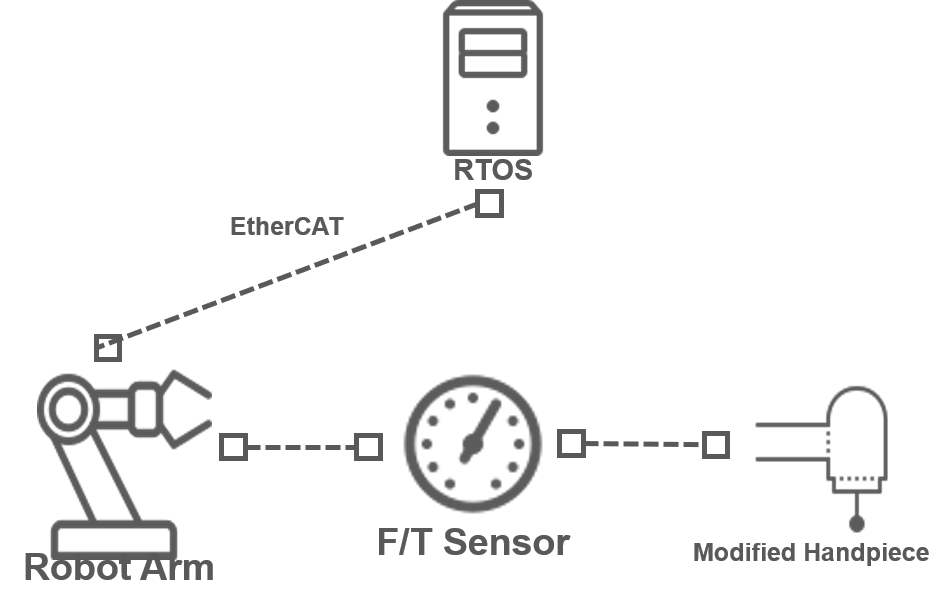
\includegraphics[width=0.7\linewidth]{Images/EtherCAT.png}
\caption{Communication protocol - EtherCAT. Master device is RT-target and slave devices are robot arm, F/T sensor and modified handpiece.}
\label{fig:EtherCAT}

\end{center}
\end{figure}
\par
In Fig \ref{fig:system}, a motion capture system was incorporated to obtain the position information \cite{web8}. There are four cameras with high resolution sensor around the robot. It can capture LEDs and calculate their Cartesian position for $960$ frames per second and its resolution is around $1$ mm. Moreover, a Stewart Platform on which a root acrylic model is mounted was set up to simulate a small patient moving. To record the handpiece and root positions, a LED marker is located on the driller and other three LED markers forming a equilateral triangle are seated on the Stewart platform and. Therefore, the handpiece position is directly obtained and the root position is calculated as following equation
\begin{equation*}
\begin{split}
p_{root} = \frac{p_{1} + p_{2} + p_{3}}{3}
\end{split}
\end{equation*}
where $p_{root}$ denotes the root position and $p_{i}$ denote the positions of LEDs obtained from the motion capture system. 
\par
Note that there is a vertical distance between the root and handpiece in this setup and an error come from inaccurate 3-D print support used to stick three LEDs. Besides, once less than three cameras concurrently capture a LED due to the shooting angle, the position information will be incorrect.  
\begin{figure}[htbp]
\begin{center}
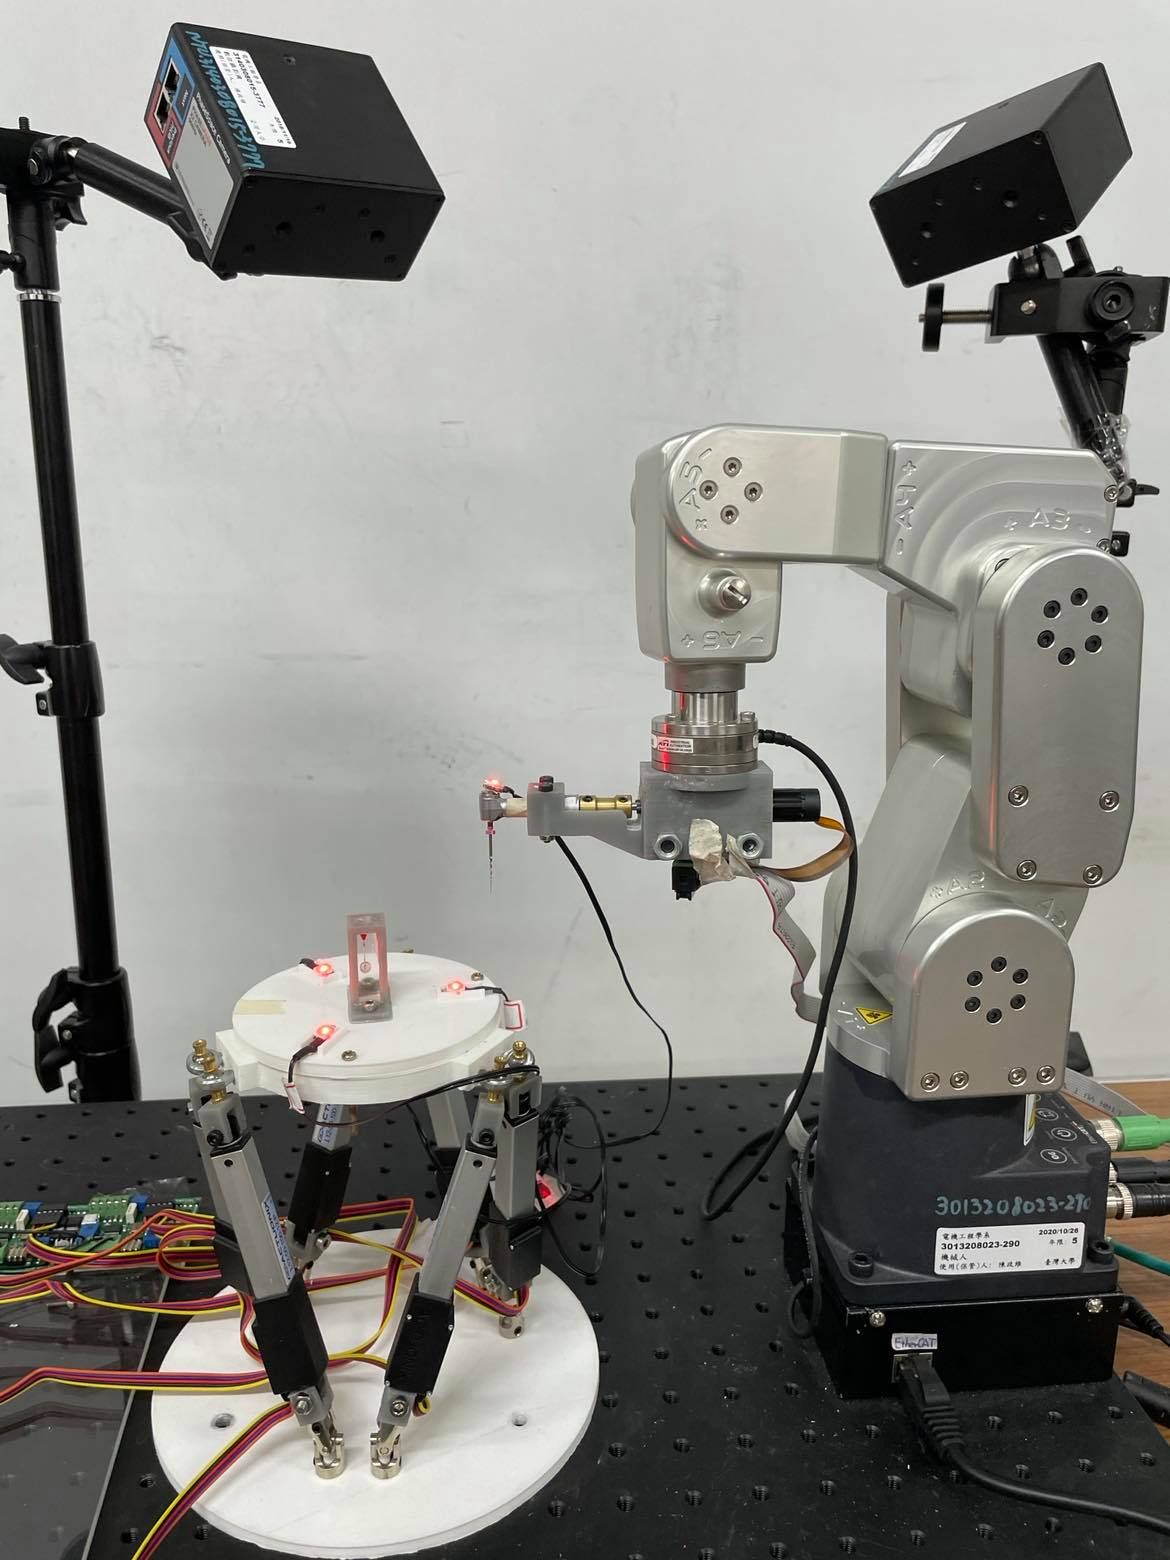
\includegraphics[width=0.7\linewidth]{Images/System.jpg}
\caption{Experimental setup with Dentibot, a motion capture system, and a Stewart platform}
\label{fig:system}
\end{center}
\end{figure}
\par
The specifications of the hardware and software environment set in the experiments are listed in Table \ref{tab:exp_specification}. Graph user interface and fundamental framework are constructed to reduce and eliminate the developing problems.  The detail specifications of the robot arm and F/T sensor are shown in Table \ref{tab:meca_specification} and Table \ref{tab:mini40_specification}.

\begin{table}[htbp]
\centering
\caption{Specifications of the hardware and software environments}
\label{tab:exp_specification}
\par
\begin{tabular}{|c|c|} 
\hline
Item											&Specification					\\	\hline
Development Environment							&LabVIEW 2018					\\	\hline
\multirow{2}{*}{Real-Time Operating System}		&National Instrument-RT target	\\
												&CPU: Intel Core 8				\\	\hline
Communication Protocol							&EtherCAT						\\	\hline
Robot Arm										&Mecademic-Meca500				\\	\hline
F/T Sensor										&ATI-Mini40						\\	\hline
\multirow{2}{*}{Handpiece Motor}							&Maxon - servo motor				\\
												&Gear ratio: 67					\\	\hline
\multirow{2}{*}{Motion Capture System}			&PhaseSpace-Impulse X2E 		\\
												&Resolution: 1mm				\\	\hline
Stewart Platform								&Actuoanix - Linear Actuator				\\	
\hline
\end{tabular}
\end{table}

\begin{figure}[htbp]
\begin{center}
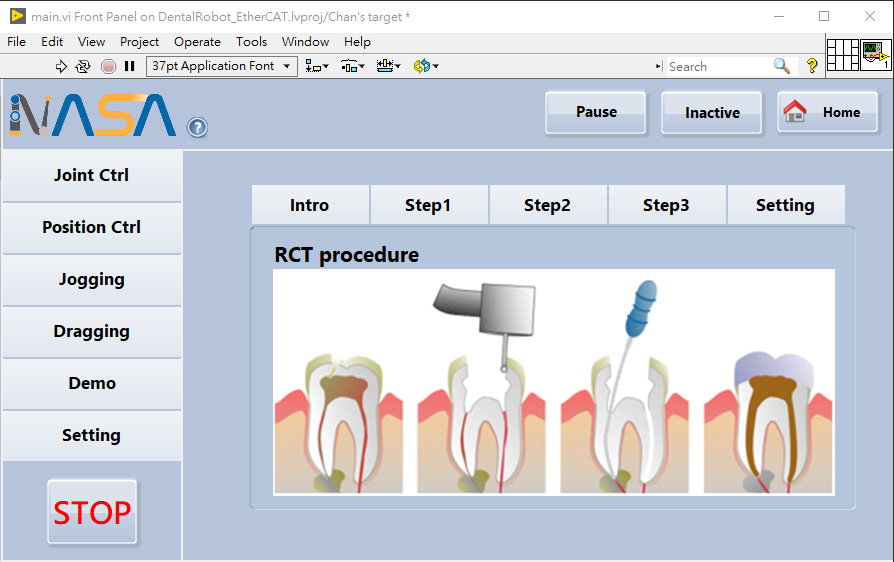
\includegraphics[width=1\linewidth]{Images/GUI.png}
\caption{Graph user interface with LabVIEW 2018}
\label{fig:GUI}
\end{center}
\end{figure}
\begin{table}[htbp]
\centering
\caption{Technical specifications of the robot arm - meca500}
\label{tab:meca_specification}
\par
\begin{tabular}{|c|c|} 
\hline
Payload						&0.5 kg					\\	\hline
Repeatability				&0.005 mm					\\	\hline
Reach (at wrist center)		&260 mm	\\ \hline
Total weight				&4.5 kg						\\	\hline
\multirow{6}{*}{Joint range}&joint 1: −175° to +175°				\\	
							&joint 2: −70° to +90°				\\	
							&joint 3: −135° to +70°				\\	
							&joint 4: −170° to +170°				\\	
							&joint 5: −115° to +115°				\\	
							&joint 6: ±100 revolutions				\\	\hline
Speed of joints 1–6 &{150, 150, 180, 300, 300, 500} °/s				\\	\hline
Brakes 				&on joints 1, 2 and 3				\\	\hline
Robot mounting 		&any orientation				\\	\hline
Safety module		&Category 3, PL d				\\	\hline
Power supply 		&90-264 VAC, 50-60 Hz (in) / 24 VDC (out)				\\	\hline
Communication 		&TCP/IP, EtherCAT, Ethernet/IP				\\	\hline
Controller 			&embedded in robot base				\\	\hline
Protection rating 	&IP 40								\\	
\hline
\end{tabular}
\end{table}

\begin{table}[htbp]
\centering
\caption{Technical specifications of the F/T sensor - mini40}
\label{tab:mini40_specification}
\par
\begin{tabular}{|c|c|} 
\hline
Weight										&0.0499 kg	\\  \hline
Diameter									&40 mm  	\\ 	\hline
Height										&12.2 mm 	\\	\hline
\multirow{4}{*}{Sensing range}					&Fx,Fy: 20 N\\
											&Fz: 60 N\\
											&Tx,Ty: 1 Nm\\	
											&Tz: 1 Nm\\	\hline
\multirow{4}{*}{Resolution}						&Fx,Fy: 1/100 N	\\
											&Fz: 1/50 N\\
											&Tx,Ty: 1/4000 Nm\\	
											&Tz: 1/4000 Nm\\	\hline										
\multirow{4}{*}{Single-axis overload} 			&Fxy: ±810 N  \\	
											&Fz	±2400 N  \\
											&Txy	±19 Nm  \\
											&Tz	±20 Nm  \\ \hline
\multirow{4}{*}{Stiffness (calculated)}   		&X-axis \& Y-axis forces (Kx, Ky): 1.1x107 N/m   \\	
											&Z-axis force (Kz): 2.0x107 N/m   \\	
											&X-axis \& Y-axis torque (Ktx, Kty): 2.8x103 Nm/rad   \\	
											&Z-axis torque (Ktz): 4.0x103 Nm/rad   \\	 \hline
\multirow{2}{*}{Resonant Frequency} 			&Fx, Fy, Tz: 3200 Hz  \\
											&Fz, Tx, Ty: 4900 Hz  \\
\hline
\end{tabular}
\end{table}

\newpage
\section{Force-Guided Alignment}
\hspace*{6mm}In order to prove the validation of force-guided alignment, we set up three experiments with different scenarios. The aim of these experiments was for validating whether it was possible that the DentiBot inserted an endodontic file into a small root and confronted a patient moving at the same time. Therefore, three experiment were designed with more and more functions.
\begin{enumerate}
\item[1.1] Inserting without file rotation
\item[1.2] Inserting with file rotation
\item[1.3] Inserting with file rotation and file feedrate control
\end{enumerate}
\par
To simulate a patient movingA Stewart platform with six degrees of freedom was incorporated. It could provide a slight movement. Basically, when the patient moved to a point, our system should move to the same place. Therefore, the target's and the handpiece's positions should be compared to check if our system tracked the patient or not. PhaseSpace - Impulse X2E was involved in obtaining the above positions in real-time. 
\par
The Stewart platform is scheduled for motion planning. It will move to (0, 0, 0), (15, 0, 0), (15, 0, 15), (0, 0, 15) related to Stewart frame with a constant velocity. These points formed a square composed of two horizontal and two vertical lines. The command position trajectory is illustrated in Fig \ref{fig: position command}. The Stewart platform is planned to go along with the square with a velocity, then stop for $10$ seconds, then go along with the square with a faster velocity, and so on. The velocities of four rounds are $3$ mm/s, $4$ mm/s, $5$ mm/s, and $6$ mm/s.
	
\begin{figure}[htbp]
\begin{center}
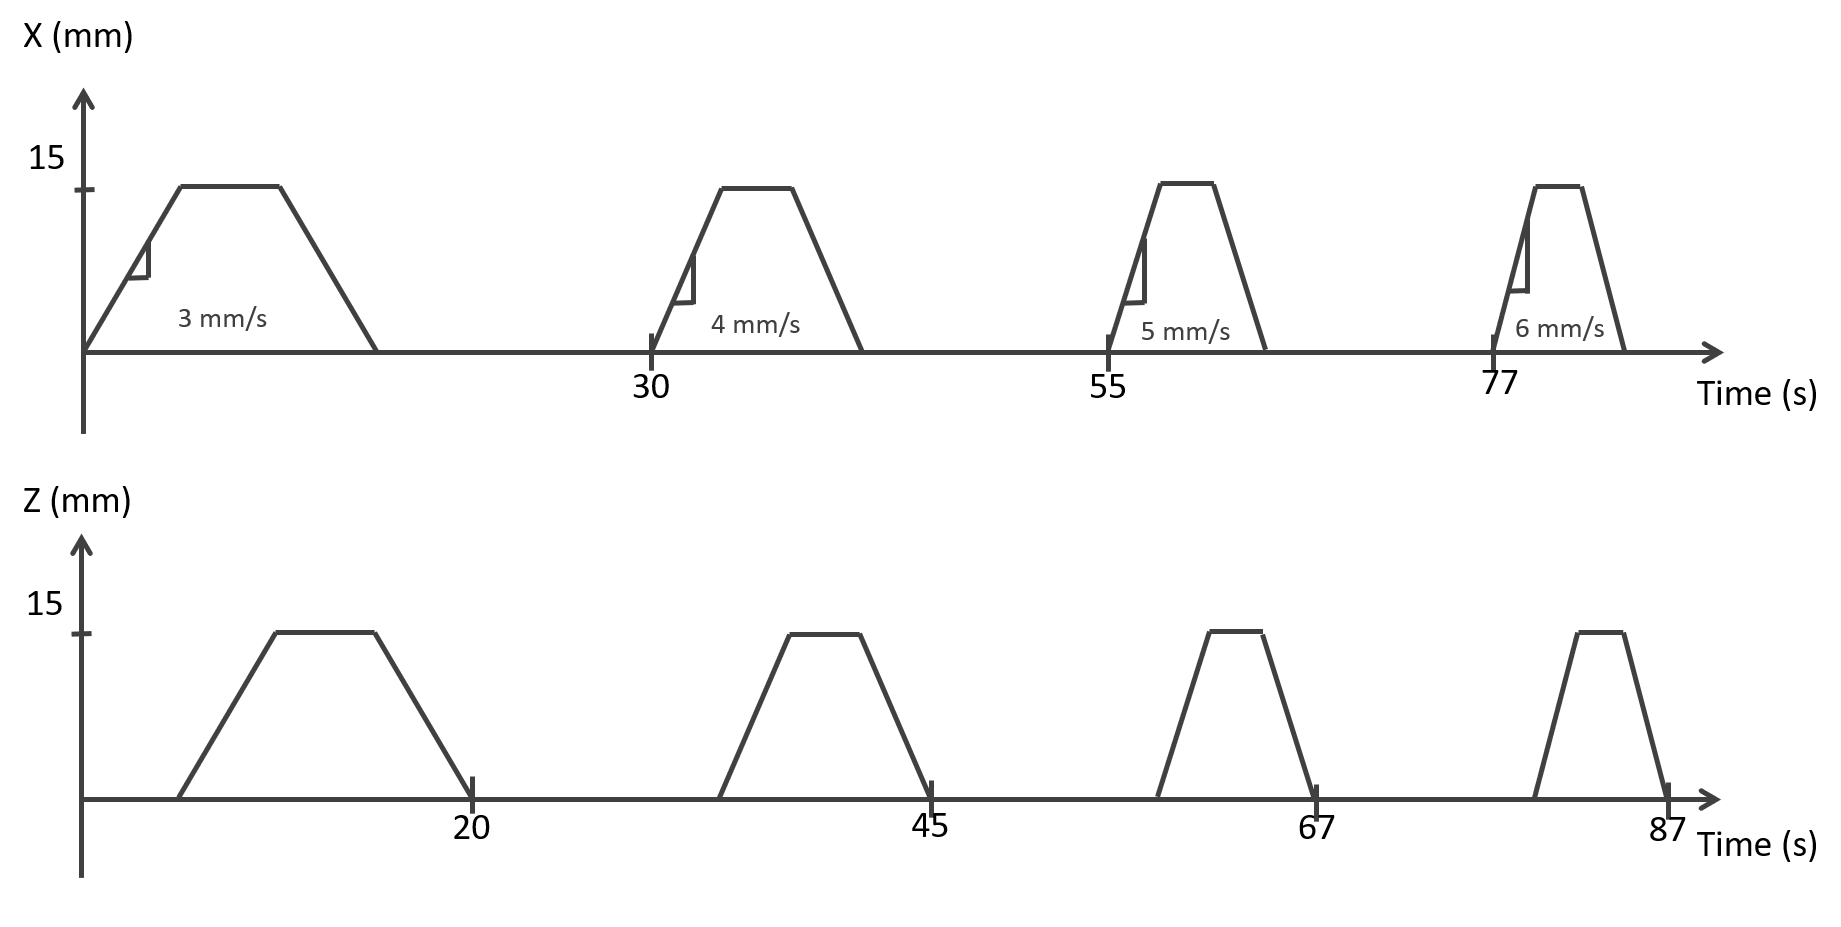
\includegraphics[width=1\linewidth]{Images/position command.png}
\caption{Position command of Stewart platform for force-guided alignment experiment}
\label{fig: position command}
\end{center}
\end{figure}	

Parameters setting of admittance control in Experiment 1. Before starting this experiment, we made the file rotate and get stuck in the root canal of an acrylic model. Then we used "Doctor dragging" mode to install the acrylic model on the Stewart platform. Therefore, we can guarantee that the relative position between the file and the acrylic tooth. The first experiment is a file without rotation 
\par
\begin{table}[htbp]
\centering
\caption{Parameters setting of admittance control in Experiment 1.}
\label{tab: para_adm_exp1}
\begin{tabular}{cccc} 
\hline \hline
Parameter	&1-1		&1-2		&1-3	\\
\hline
$k$			&$500$		&$500$		&$500$				\\
$f_z$		&$1$		&$1$		&$-0.5 \sim 0.5$	\\
$b_1$		&$80$		&$80$		&$80$				\\
$b_2$		&$80$		&$80$		&$80$				\\
$b_3$		&$80$		&$80$		&$80$				\\
$b_4$		&$80$		&$80$		&$80$				\\
$b_5$		&$80$		&$80$		&$80$				\\
$b_6$		&$80$		&$999999$	&$999999$			\\
\hline	
\multicolumn{4}{*}{$\mathbf{K} = \text{diag}(k,k,k,k,k,k),\mathbf{B} = \text{diag}(b_1,b_2,b_3,b_4,b_5,b_6)$}\\
\hline\hline	
\end{tabular}
\end{table}
We moved the Stewart platform in horizontal and vertical directions separately. The motion planning in the horizontal direction is a square which is $10\times 10$ mm and in the vertical direction is a linear motion from $0$ to $40$ mm.
\section{Pre-Clinical Trial}
Validation of Self-alignment Mode
\par\noindent
(Metrics: time, completeness and file breakage)								
\par\noindent
(Completeness definition: comparison of pixel area before and after experiment via image)
validation of repetitive experiment
\par\noindent
(Metrics: file breakage, compare with and without reverse)